\documentclass[oneside, a4paper]{article}

\usepackage[left=25mm, right=25mm, top=25mm, bottom=25mm, paper=a4paper]{geometry}
\usepackage[utf8]{inputenc}
\usepackage[spanish]{babel}
\usepackage{csquotes}
\usepackage{float}
\usepackage{hyperref}
\usepackage{tabularx}
\usepackage{array}
\usepackage{graphicx}
\usepackage{fancyhdr}
\usepackage{amsmath}
\usepackage{amssymb}
\usepackage{multicol}


\graphicspath{{./../img/}}
\fancyhf{}
\fancyhead[L]{
\includegraphics[scale=0.15]{espe.png}}
\fancyhead[R]{
\includegraphics[scale=0.05]{ciencias_de_computacion.jpg}}
\setlength{\headheight}{50pt}
\setlength{\parindent}{0pt}

\title{
    \Large
    \begin{center}
        \includegraphics*[scale=0.3]{espe.png}
    \end{center}
    \textbf{UNIVERSIDAD DE LAS FUERZAS ARMADAS ESPE}\\
    \textbf{DEPARTAMENTO DE CIENCIAS DE LA COMPUTACIÓN}\\
    \textbf{INGENIERÍA DE SOFTWARE}
}
\author{\\
    \textbf{NRC:} 14774\\
    \textbf{Materia:} Computación Gráfica\\
    \textbf{Tema:} Aplicaciones de Computación Gráfica\\\\
    \textbf{Grupo 2}\\
    Albán Richard\\
    Escobar Aymé\\
    Guacán Alexander\\
    Macas Karol\\\\\\\\
    Ing. César Javier Villacís Silva
}
\date{}

\begin{document}
    \pagestyle{fancy}

    \begin{titlepage}
        \maketitle
    \end{titlepage}

    \section{Descripción del problema}
        Dado el lado de un pentágono, dibujar la figura geométrica correspondiente y los diferentes polígonos estrellados de 5 puntas, tal y como se muestra en la Figura \ref{fig:star_pentagon}. Se debe considerar que las figuras geométricas se grafican con respecto al punto $O(0,0)$.

        \begin{figure}[H]
            \centering
            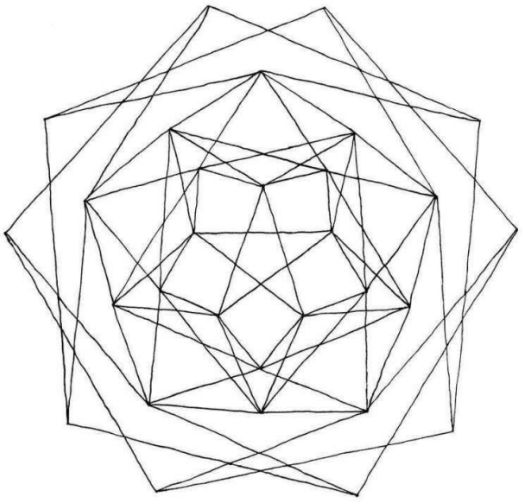
\includegraphics[scale=0.5]{star_pentagon.png}
            \caption{Péntagono y polígonos estrellados de 5 puntas.}
            \label{fig:star_pentagon}
        \end{figure}

    \section{Geometría de la figura}
        \subsection{Pentágono}
            La figura principal para lograr solucionar el problema es el pentágono. Para graficarlo se ha optado por utilizar la intersección de un círculo circunscrito al pentágono y rectas que tienen una separación de $72^{\circ}$ como se ve en la Figura \ref{fig:pentagon}, que es la medida de su ángulo central $\alpha$. Cada una de estas intersecciones representa los vértices del pentágono. De esta manera, si deseamos que el pentágono esté paralelo al eje Y, bastará con sumar un ángulo inicial a la recta del primer vértice para conseguirlo. Además otro ángulo conocido es el ángulo interno del pentágono que es de $108^{\circ}$, donde cada línea de intersección con el círculo también es una bisectriz, por lo tanto $\beta = 54^{\circ}$.

            \begin{figure}[H]
                \centering
                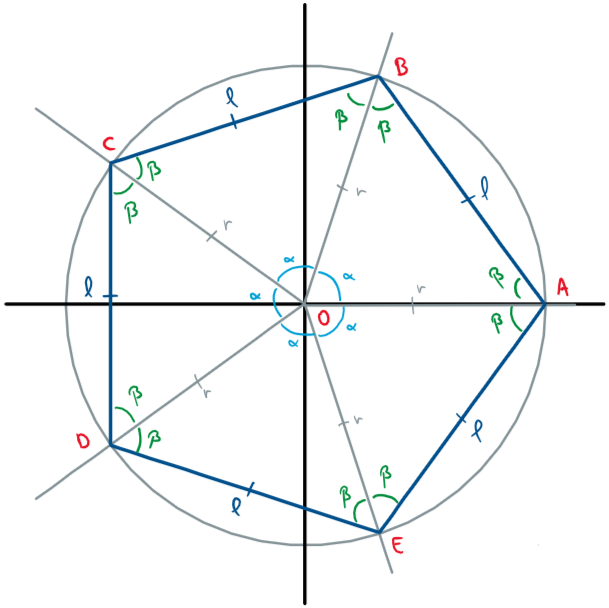
\includegraphics[scale=0.5]{pentagon.png}
                \caption{Vértices, ángulos y lados del hexágono.}
                \label{fig:pentagon}
            \end{figure}

            Comenzaremos obteniendo la fórmula general para poder calcular el radio del círculo circunscrito dado la medida del lado del pentágono:
            
            \begin{figure}[H]
                \centering
                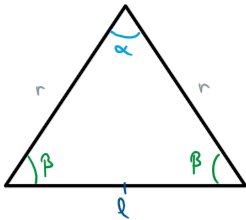
\includegraphics[scale=0.5]{internal_triangle.png}
                \caption{Triángulo interno del pentágono.}
                \label{fig:internal_triangle}
            \end{figure}

            Ley de senos:

            \begin{align}
                \frac{r}{\sin(\beta)} & = \frac{l}{\sin(\alpha)} \nonumber  \\
                r                     & = l\frac{\sin(\alpha)}{\sin(\beta)}
                \label{eq:radius_circumscribed_circle}
            \end{align}

            Procederemos a obtener la fórmula general para calcular el punto de intersección entre el círculo circunscrito y la recta dado un ángulo $\theta$, este ángulo representará el ángulo de separación $\alpha$ entre cada uno de los vértices. Recordemos que:

            \begin{align}
                y - y_{1}             & = m(x - x_{1}) \label{eq:general_equation_straight_line} \\
                m                     & = tan(\theta) \label{eq:slope}                           \\
                (x - h)^2 + (y - k)^2 & = r^2 \label{eq:general_equation_circle}
            \end{align}

            Dado que cualquier recta pasará por el centro $(h, k)$ de la circunferencia, y que la pendiente de la recta esta en función de su ángulo, remplazamos (\ref{eq:slope}) en (\ref{eq:general_equation_straight_line}):

            \begin{align}
                y - k & = tan(\theta)(x - h) \nonumber                                     \\
                y     & = tan(\theta)(x - h) + k \label{eq:straight_line_in_center_circle}
            \end{align}

            Remplazamos (\ref{eq:straight_line_in_center_circle}) en (\ref{eq:general_equation_circle}):

            \begin{align*}
                (x - h)^2 + [tan(\theta)(x - h) + k - k]^2 & = r^2 \\
                (x - h)^2 + tan^2(\theta)(x - h)^2         & = r^2 \\
                [1 + tan^2(\theta)](x - h)^2               & = r^2
            \end{align*}

            Por identidad trigonométrica sabemos que:

            \begin{align}
                1 + tan^2(\theta) & = \sec^2(\theta)\label{eq:tan2_trigonometric_identity}                   \\
                sec^2(\theta)     & = \frac{1}{cos^2(\theta)}\label{eq:sec_trigonometric_identity}           \\
                tan(\theta)       & = \frac{\sin(\theta)}{\cos(\theta)}\label{eq:tan_trigonometric_identity}
            \end{align}

            Por lo tanto, remplazando con (\ref{eq:tan2_trigonometric_identity}) y (\ref{eq:sec_trigonometric_identity}):

            \begin{align*}
                (x - h)^2\sec^2(\theta)             & = r^2               \\
                \sec^2(\theta)(x^2 - 2hx + h^2)     & = r^2               \\
                x^2 - 2hx + h^2                     & = r^2\cos^2(\theta) \\
                x^2 - 2hx + h^2 - r^2\cos^2(\theta) & = 0                 \\
            \end{align*}

            Calculamos las raices:

            \begin{align}
                x_{1,2} & = \frac{-b \pm \sqrt{b^2 - 4ac}}{2a}\nonumber                            \\
                x_{1,2} & = \frac{2h \pm \sqrt{4h^2 - 4[h^2 - r^2\cos^2(\theta)]}}{2}\nonumber     \\
                x_{1,2} & = \frac{2h \pm \sqrt{4[h^2 - h^2 + r^2\cos^2(\theta)]}}{2}\nonumber      \\
                x_{1,2} & = \frac{2h \pm \sqrt{4r^2\cos^2(\theta)}}{2}\nonumber                    \\
                x_{1,2} & = \frac{2h \pm 2r\cos(\theta)}{2}\nonumber                               \\
                x       & = h + r\cos(\theta)\label{eq:coordinate_root_intersection_line_circle}
            \end{align}

            Solo tomaremos la ecuación con signo positivo, ya que el ángulo que corresponde al vértice del pentágono es positivo. Por lo tanto, remplazando (\ref{eq:coordinate_root_intersection_line_circle}) y (\ref{eq:tan_trigonometric_identity}) en (\ref{eq:straight_line_in_center_circle}), obtenemos:

            \begin{align*}
                y & = \tan(\theta)[h + rcos(\theta) - h] + k             \\
                y & = rcos(\theta)\tan(\theta) + k                       \\
                y & = r\cos(\theta)\frac{\sin(\theta)}{\cos(\theta)} + k \\
                y & = k + r\sin(\theta)                                  \\
            \end{align*}

            Por lo tanto los vértices del pentagono en función de su ángulo de inclinación son:

            \begin{equation}
                \begin{aligned}
                    O(x, y) & = O(h, k)                                   \\
                    A(x, y) & = A(h + r, b)                               \\
                    B(x, y) & = B(h + r\cos(\alpha), k + r\sin(\alpha))   \\
                    C(x, y) & = C(h + r\cos(2\alpha), k + r\sin(2\alpha)) \\
                    D(x, y) & = D(h + r\cos(3\alpha), k + r\sin(3\alpha)) \\
                    E(x, y) & = E(h + r\cos(4\alpha), k + r\sin(4\alpha)) \\
                \end{aligned}
                \label{eq:pentagon_vertices}
            \end{equation}

            Con los vértices de (\ref{eq:pentagon_vertices}), podemos graficar el primer pentágono, pero si deseamos graficar el pentágono paralelo al eje $y$, requerimos de un ángulo más que nos indique el ángulo inicial de inclinación como se puede observar en la Figura \ref{fig:vertical_pentagon}.

            \begin{figure}[H]
                \centering
                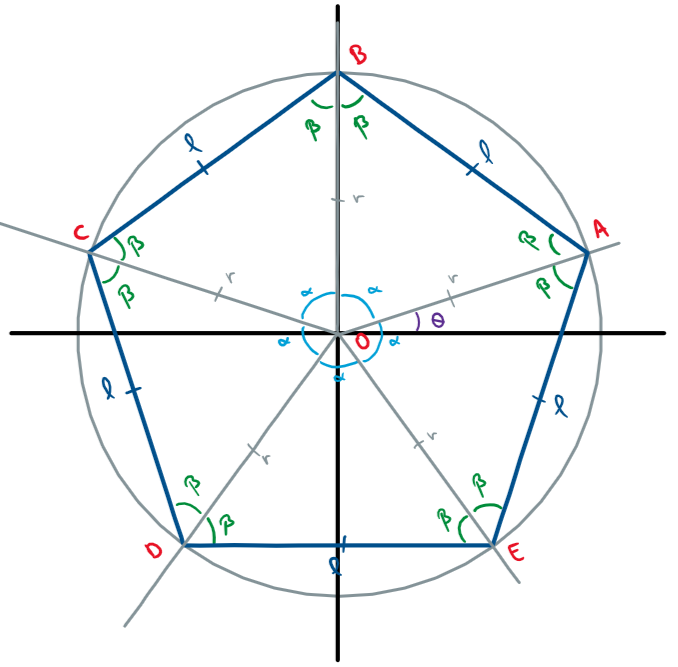
\includegraphics[scale=0.5]{vertical_pentagon.png}
                \caption{Pentágono vertical.}
                \label{fig:vertical_pentagon}
            \end{figure}

            Calculamos el ángulo $\theta$ para el pentagono de la Figura \ref{fig:vertical_pentagon}:

            \begin{align}
                \alpha + \theta & = 90 \nonumber\\
                \theta & = 90 - 72 \nonumber\\
                \theta & = 18 \label{eq:theta_angle_vertical_pentagon}
            \end{align}

            Calculamos el ángulo $\theta$ para el pentágono de la Figura \ref{fig:pentagon_tilted_left}:

            \begin{figure}[H]
                \centering
                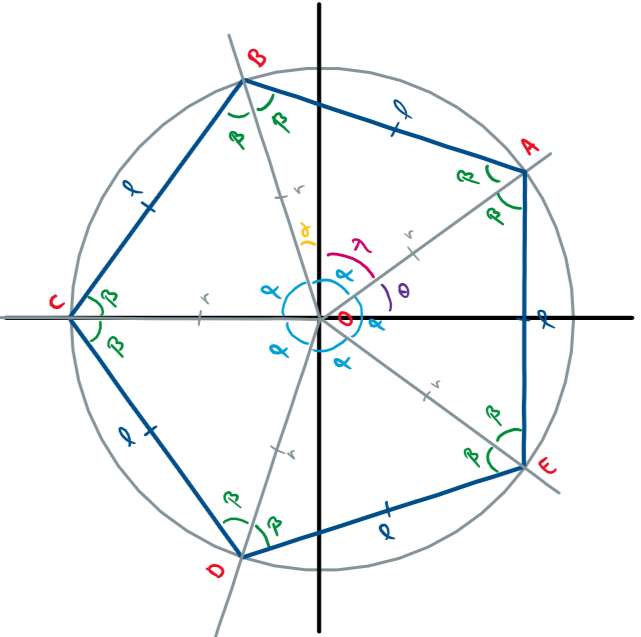
\includegraphics[scale=0.5]{pentagon_tilted_left.png}
                \caption{Pentágono vertical.}
                \label{fig:pentagon_tilted_left}
            \end{figure}

            Sabemos que:

            \begin{align}
                \alpha + \gamma  & = 90\label{eq:theorem1_pentagon_tilted_left}     \\
                \gamma + \lambda & = \alpha\label{eq:theorem2_pentagon_tilted_left} \\
                \theta + \lambda & = 90\label{eq:theorem3_pentagon_tilted_left}
            \end{align}

            Despejamos $\alpha$ de (\ref{eq:theorem1_pentagon_tilted_left}):

            \begin{align}
                \alpha + \gamma & = 90 \nonumber\\
                \alpha & = 90 - 72 \nonumber\\
                \alpha & = 18 \label{eq:alpha_angle}
            \end{align}

            Remplazamos (\ref{eq:alpha_angle}) en (\ref{eq:theorem2_pentagon_tilted_left}):

            \begin{align}
                \gamma + \lambda & = \alpha \nonumber\\
                \lambda & = 72 - 18 \nonumber\\
                \lambda & = 54 \label{eq:lambda_angle}
            \end{align}

            Por lo tanto, al remplazar (\ref{eq:lambda_angle}) en (\ref{eq:theorem3_pentagon_tilted_left}):

            \begin{align}
                \theta + \lambda & = 90 \nonumber\\
                \theta & = 90 - 54 \nonumber\\
                \theta & = 36 \label{eq:theta_angle_pentagon_tilted_left}
            \end{align}

        \subsection{Pentágono central}
            Una vez graficamos los pentágonos de la Figura \ref{fig:pentagon} y \ref{fig:pentagon_tilted_left}. Debemos graficar el pentágono central de la Figura \ref{fig:center_pentagon}, para ello podemos observar que el vértice superior es paralelo a una de las intersecciones $I$ de los pentágonos externos, esto significa que la distancia entre la coordenada $x_{I}$ y el origen, es el radio de la circunferencia circunscrita al pentágono central.

            \begin{figure}[H]
                \centering
                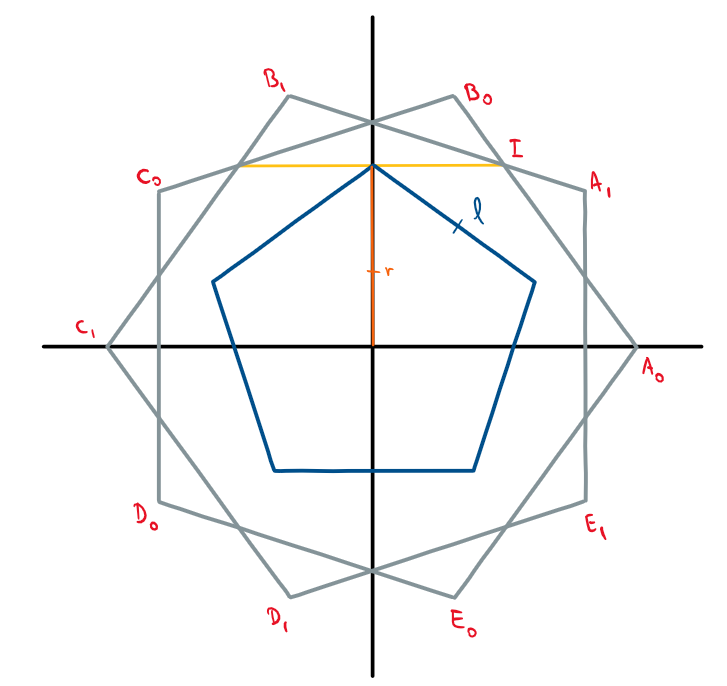
\includegraphics[scale=0.5]{center_pentagon.png}
                \caption{Pentágono central a la figura.}
                \label{fig:center_pentagon}
            \end{figure}

            Por lo tanto, el radio del pentágono central es:

            \begin{equation}
                r = |y_{I} - y_{O}|
                \label{eq:radius_center_pentagon}
            \end{equation}

            Para encontrar el punto $I$ haremos uso del teorema del punto medio entre dos rectas:
            
            \begin{equation}
                Pm(x, y) = Pm(\frac{y_{3} - y_{1} + m_{1}x_{1} - m_{2}x_{3}}{m_{1} - m_{2}}, y_{1} + m_{1}(x_{Pm} - x_{1}))
                \label{eq:intersection_point_between_straight_lines}
            \end{equation}

            Donde:

            \begin{align*}
                m_{1} & = \frac{y_{2} - y_{1}}{x_{2} - x_{1}}\\
                m_{2} & = \frac{y_{4} - y_{3}}{x_{4} - x_{3}}
            \end{align*}

            Entonces, si despejamos $l$ de la Ecuación (\ref{eq:radius_circumscribed_circle}), obtenemos que el lado del pentágono central es:

            \begin{equation}
                l = r\frac{\sin(\alpha)}{\sin{\beta}}
                \label{eq:pentagon_side}
            \end{equation}

        \subsection{Unión de vértices pentágonos externos y pentágono central}
            En la Figura \ref{fig:union_external_to_internal_pentagons} se ilustra como se une cada uno de los vertices de ambos pentágonos externos con el pentágono central. Aquí podemos darnos cuenta que el pentágono de la Figura \ref{fig:pentagon}, une cada uno de sus vértices con el anterior vértice al del pentágono central. Por el contrario, el pentágono de la Figura \ref{fig:pentagon_tilted_left} une cada vértice con el siguiente vértice del pentágono central.
            
            \begin{figure}[H]
                \centering
                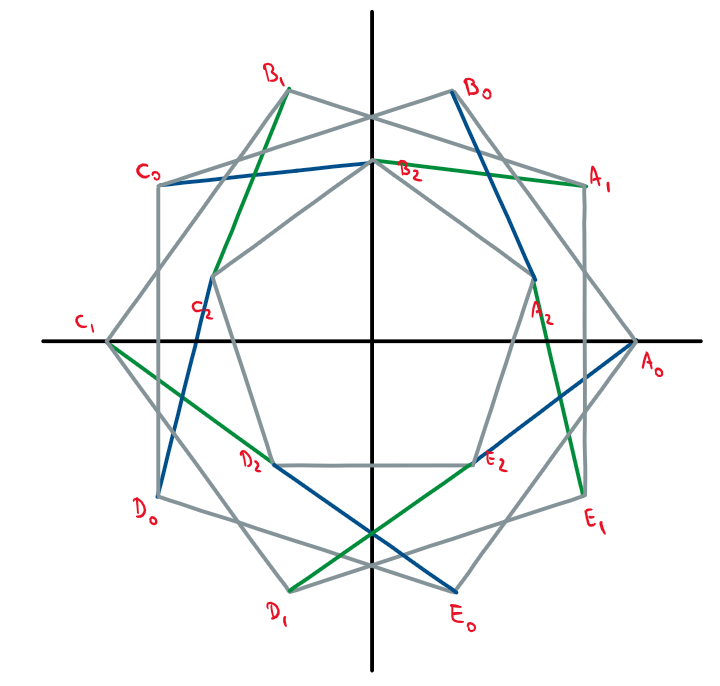
\includegraphics[scale=0.5]{union_external_to_internal_pentagons.png}
                \caption{Unión de vértices entre pentágonos externos y pentágono central.}
                \label{fig:union_external_to_internal_pentagons}
            \end{figure}

            Entonces, lo que haremos será calcular los segmentos $\overrightarrow{P_{0}P_{2}}$ y $\overrightarrow{P_{1}P_{2}}$ que une los vertices $P_{0}$ del pentágono con un grado de inclinación $\theta = 0^{\circ}$, con los vértices $P_{2}$ del pentágono central, y de los vértices $P_{1}$ del pentágono con $\theta = 36^{\circ}$ con el pentágono central, respectivamente.

            \begin{equation}
                \overrightarrow{P_{0}P_{2}}[i] =
                \begin{cases}
                    P_{o}[i] = P_{0}[i] \\
                    P_{f}[i] = P_{2}[(5 + i - 1) \: \textrm{mod} \: 5]
                \end{cases}
                \textrm{, } D = \{ i \: \epsilon \: \mathbb{N} \: | \: 0 \leqslant i \leqslant 4 \}
                \label{eq:union1_vertices_internal_external_pentagon}
            \end{equation}
            
            \begin{equation}
                \overrightarrow{P_{1}P_{2}}[i] =
                \begin{cases}
                    P_{o}[i] = P_{1}[i] \\
                    P_{f}[i] = P_{2}[(5 + i + 1) \: \textrm{mod} \: 5]
                \end{cases}
                \textrm{, } D = \{ i \: \epsilon \: \mathbb{N} \: | \: 0 \leqslant i \leqslant 4 \}
                \label{eq:union2_vertices_internal_external_pentagon}
            \end{equation}

            La iteración de $i$ representa a cada vértice de los pentágonos, donde $A = 0$, $B = 1$ y así sucesivamente. Además, la palabra \textit{mod} representa el módulo o residuo entre la división de los operandos izquierdo y derecho a este operador.

        \subsection{Unión vértices y puntos medios del pentágono central}
            La siguiente parte del gráfico es la unión de los vértices del pentágono central con dos puntos medios de los lados de este pentágono. En la Figura \ref{fig:vertex_to_median_connection}, se puede visualizar la conexión de cada uno de estas medianas. Así que, primero deberemos calcular los puntos medios de cada uno de los lados del pentágono.

            \begin{figure}[H]
                \centering
                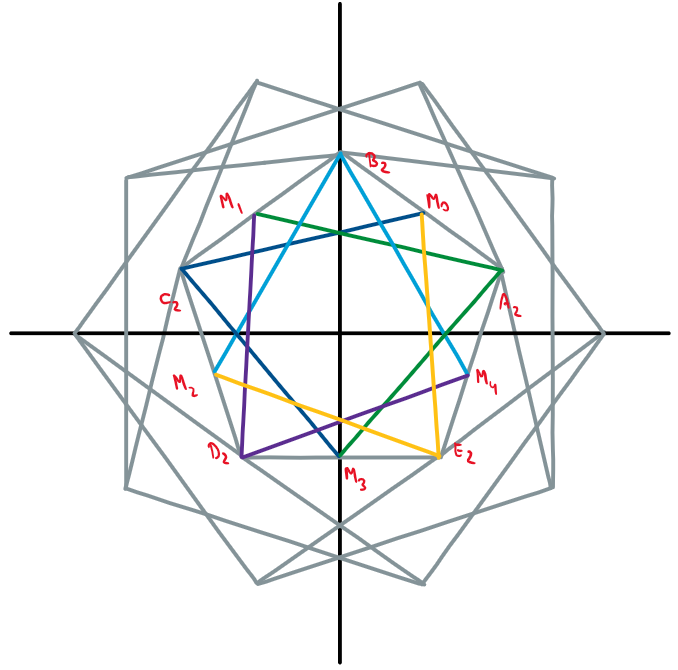
\includegraphics[scale=0.5]{vertex_to_median_connection.png}
                \caption{Unión de vértices y puntos medios del pentágono central.}
                \label{fig:vertex_to_median_connection}
            \end{figure}

            Ecuación del punto medio:

            \begin{equation}
                M(x, y) = M(\frac{x_{1} + x_{2}}{2}, \frac{y_{1} + y_{2}}{2})
                \label{eq:middle_point}
            \end{equation}

            Puntos medios del pentágono:

            \begin{equation}
                M_{i}(x, y) = M_{i}(\frac{x_{i} + x_{(5 + i + 1) \: \textrm{mod} \: 5}}{2}, \frac{y_{i} + y_{(5 + i + 1) \: \textrm{mod} \: 5}}{2}) \textrm{, } D = \{ i \: \epsilon \: \mathbb{N} \: | \: 0 \leqslant i \leqslant 4 \}
                \label{eq:middle_points_pentagon}
            \end{equation}
            
            Lo que podemos notar es que, para cada vértice, se conecta con el punto medio del siguiente lado adyacente al vértice en sentido horario y también en sentido antihorario. Por ejemplo, para el vértice $A_{2}$, su lado adyacente en sentido antihorario es $\overrightarrow{A_{2}B_{2}}$, y en sentido horario es $\overrightarrow{A_{2}E_{2}}$, por lo que su unión se dá con el lado $\overrightarrow{B_{2}C_{2}}$ y $\overrightarrow{D_{2}E_{2}}$, respectivamente.

            Por lo tanto, la ecuación que replica este patrón para cada uno de los segmentos $\overrightarrow{P_{2}M}$ en sentido antihorario es:

            \begin{equation}
                \overrightarrow{P_{2}M}[i] =
                \begin{cases}
                    P_{o}[i] = P_{2}[i] \\
                    P_{f}[i] = M[(5 + i + 1) \: \textrm{mod} \: 5]
                \end{cases}
                \textrm{, } D = \{ i \: \epsilon \: \mathbb{N} \: | \: 0 \leqslant i \leqslant 4 \}
                \label{eq:union1_vertices_medians_central_pentagon}
            \end{equation}
            
            Sentido horario:
            
            \begin{equation}
                \overrightarrow{P_{2}M}[i] =
                \begin{cases}
                    P_{o}[i] = P_{2}[i] \\
                    P_{f}[i] = M[(5 + i - 2) \: \textrm{mod} \: 5]
                \end{cases}
                \textrm{, } D = \{ i \: \epsilon \: \mathbb{N} \: | \: 0 \leqslant i \leqslant 4 \}
                \label{eq:union2_vertices_medians_central_pentagon}
            \end{equation}

        \subsection{Estrella de 5 puntas}

            El último polígono que queda por dibujar es la estrella de 5 puntas. Para graficarla, como se puede observar en la Figura \ref{fig:five_pointed_star}, debemos hacerlo utlizando los vértices de un pentágono. Una estrella de este tipo se puede graficar utilizando un único trazo, conectando en un orden específico cada vértice. Podemos comenzar desde cualquier vértice, en este caso empezaremos desde le vértice $A$, por lo tanto, el orden de los vértices es: A, C, E, B, D, A.

            \begin{figure}[H]
                \centering
                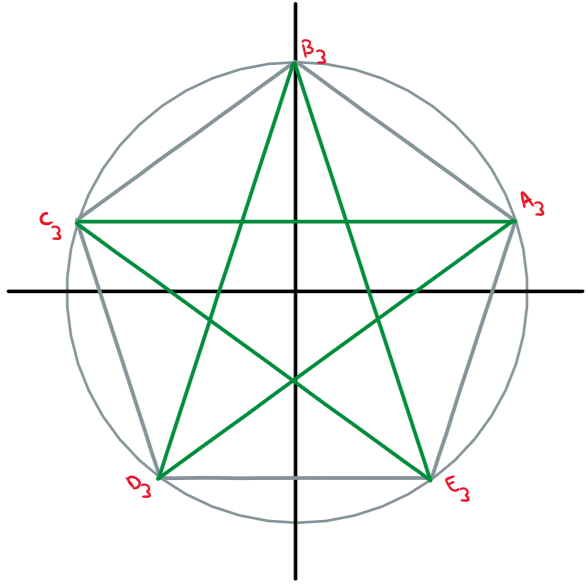
\includegraphics[scale=0.5]{five_pointed_star.png}
                \caption{Estrella de 5 puntas.}
                \label{fig:five_pointed_star}
            \end{figure}

            El patrón a seguir para graficar la estrella, es unir un vértice con el siguiente vértice saltandose uno en sentido antihorario, esto se hace hasta que se vuelva a conectar con el vértice desde donde empezamos a dibujar.

            Unión de vértices de un pentágono para dibujar estrella de 5 puntas partiendo desde cualquier vértice:
            
            \begin{equation}
                \overrightarrow{{P_{3}}_{o}{P_{3}}_{f}}[i] =
                \begin{cases}
                    P_{o}[i] = P_{3}[i] \\
                    P_{f}[i] = P_{3}[(5 + i - 2) \: \textrm{mod} \: 5]
                \end{cases}
                \textrm{, } D = \{ i \: \epsilon \: \mathbb{N} \: | \: 0 \leqslant i \leqslant 5 \}
                \label{eq:five_pointed_star_vertices}
            \end{equation}

            Si observamos la Figura \ref{fig:star_pentagon}, la estrella en el centro del gráfico tiene sus vértices A y C en paralelo a los vértices A y C de los polígonos exteriores respectivamente. Dicho en otras palabras, el centro de la estrella esta trasladado en sentido vertical, donde el segmento $\overrightarrow{AC}$ está en paralelo al eje $X$ como se puede observar en la Figura \ref{fig:five_pointed_star_translated}. Por lo tanto, el valor de $h$ nos dará la medida en la que deberemos desplazar el centro de la estrella.

            \begin{figure}[H]
                \centering
                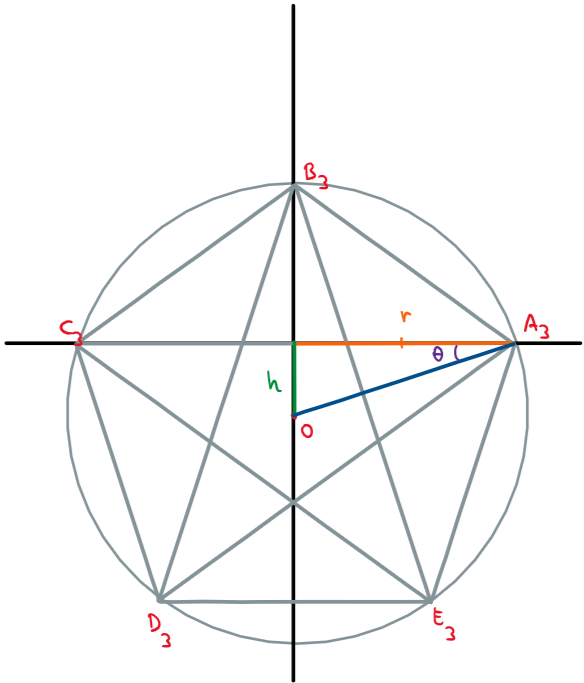
\includegraphics[scale=0.5]{five_pointed_star_translated.png}
                \caption{Estrella de 5 puntas con segmento $\overrightarrow{AC}$ paralelo al eje $X$.}
                \label{fig:five_pointed_star_translated}
            \end{figure}

            Por ángulos alternos internos:
            \begin{equation*}
                \theta = 18^{\circ}
            \end{equation*}

            Por identidad trigonométrica:

            \begin{align}
                \sin(\theta) & = \frac{h}{r} \nonumber                           \\
                h            & = {r}\sin(\theta) \label{eq:vertical_translation}
            \end{align}

            Centro de la estrella:

            \begin{equation}
                O(x, y) = O(x_{O}, y_{O} - h)
                \label{eq:five_pointed_star_center}
            \end{equation}

            Una vez que identificamos la ubicación de la estrella de 5 puntas, debemos determinar que tan grande debe ser la misma. En la Figura \ref{fig:five_pointed_star_center} vemos como los vértices $A$ y $C$ están en paralelo a las intersecciones de los segmentos que unen los vértices y medianas $\overrightarrow{A_{2}M_{1}}$, $\overrightarrow{B_{2}M_{4}}$ y $\overrightarrow{C_{2}M_{0}}$, $\overrightarrow{B_{2}M_{2}}$ respectivamente. Además por la Figura \ref{fig:five_pointed_star_translated} sabemos que la distancia del centro a el vértice $A$ o $C$, corresponde a la medida del radio de la circunferencia circunscrita.

            \begin{figure}[H]
                \centering
                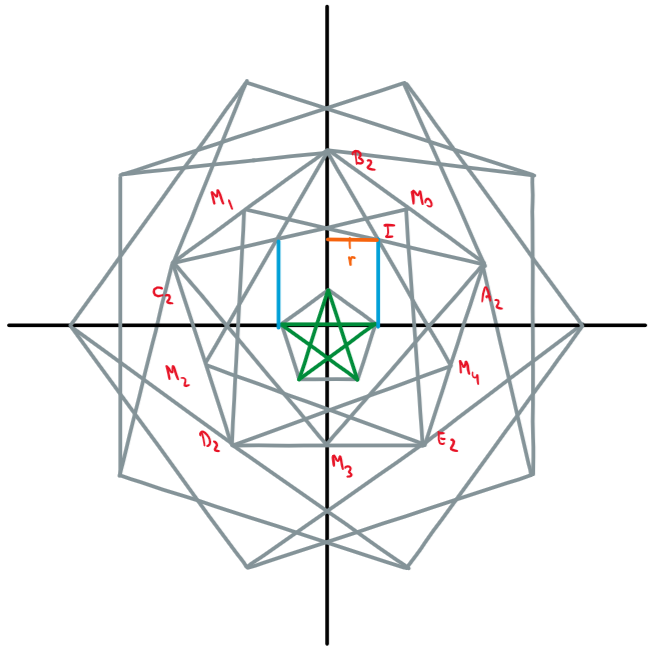
\includegraphics[scale=0.5]{five_pointed_star_center.png}
                \caption{Estrella de 5 puntas con segmento $\overrightarrow{AC}$ paralelo al eje $X$.}
                \label{fig:five_pointed_star_center}
            \end{figure}

            Entonces, usando la Ecuación (\ref{eq:intersection_point_between_straight_lines}) y (\ref{eq:pentagon_side}), utilizaremos el punto $I$ que es la intersección de los segmentos $\overrightarrow{A_{2}M_{1}}$ y $\overrightarrow{B_{2}M_{4}}$, por lo tanto, el radio de la estrella es:

            \begin{equation}
                r = |x_{I} - x_{O}|
                \label{eq:five_pointed_star_radius}
            \end{equation}

        \subsection{Unión medianas del pentágono central y vértices de la estrella}
            A continuación debemos unir cada mediana del pentágono central con dos puntas de la estrella como se ilustra en la Figura \ref{fig:star_union_to_median}.

            \begin{figure}[H]
                \centering
                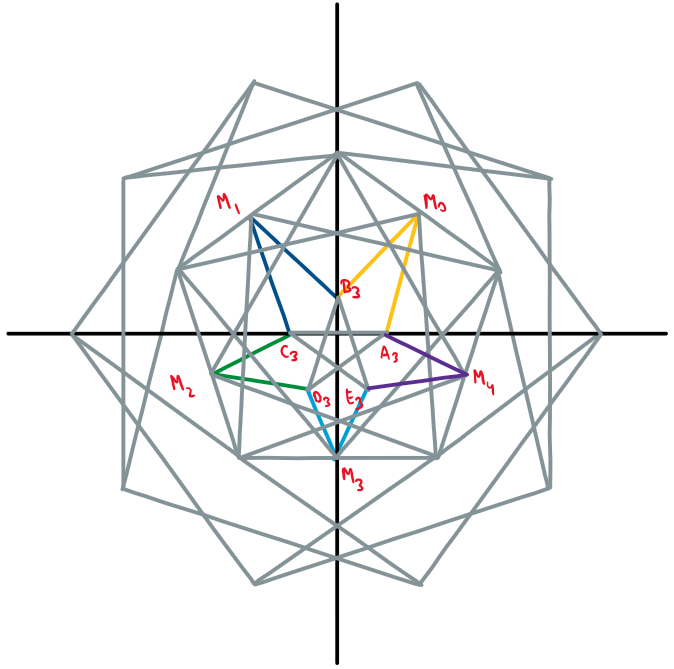
\includegraphics[scale=0.5]{star_union_to_median.png}
                \caption{Unión medianas pentágono central y puntas de estrella.}
                \label{fig:star_union_to_median}
            \end{figure}

            Función que describe la conexión de los puntos medios del pentágono central con las puntas de las estrella en orden paralelo:

            \begin{equation}
                \overrightarrow{MP_{3}}[i] =
                \begin{cases}
                    P_{o}[i] = M[i] \\
                    P_{f}[i] = P_{3}[i]
                \end{cases}
                \textrm{, } D = \{ i \: \epsilon \: \mathbb{N} \: | \: 0 \leqslant i \leqslant 4 \}
                \label{eq:union1_medians_vertices_pentagon_star}
            \end{equation}

            Función que describe la conexión de los puntos medios del pentágono central con la siguiente punta de la estrella en sentido antihorario:

            \begin{equation}
                \overrightarrow{MP_{3}}[i] =
                \begin{cases}
                    P_{o}[i] = M[i] \\
                    P_{f}[i] = P_{3}[(5 + i + 1) \: \textrm{mod} \: 5]
                \end{cases}
                \textrm{, } D = \{ i \: \epsilon \: \mathbb{N} \: | \: 0 \leqslant i \leqslant 4 \}
                \label{eq:union2_medians_vertices_pentagon_star}
            \end{equation}

        \subsection{Unión intersección de medianas del pentágono central y vértices de la estrella}
            Por último, tenemos que unir cada intersección de las medianas del pentágono central con dos puntas de la estrella como se ilustra en la Figura \ref{fig:star_union_to_median_intersections}.
            
            \begin{figure}[H]
                \centering
                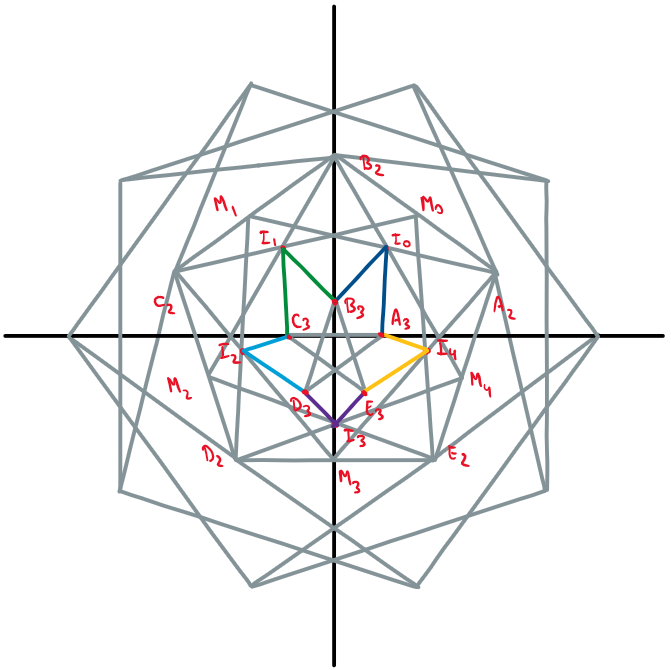
\includegraphics[scale=0.5]{star_union_to_median_intersections.png}
                \caption{Unión intersección de medianas pentágono central y puntas de estrella.}
                \label{fig:star_union_to_median_intersections}
            \end{figure}

            Utilizando la Ecuación (\ref{eq:intersection_point_between_straight_lines}), obtenemos la función para calcular las intersecciones de las medianas del pentágono central:

            \begin{equation}
                I[i](x, y) =
                \begin{cases}
                    x = Pm(\overrightarrow{P_{2}[i]M[(5 + i + 1) \: \textrm{mod} \: 5]}) \\
                    y = Pm(\overrightarrow{P_{2}[(5 + i + 1) \: \textrm{mod} \: 5]M[(5 + i + 1) \: \textrm{mod} \: 5]})
                \end{cases}
                \label{eq:intersection_median_points_central_pentagon}
            \end{equation}

            Donde:

            \begin{equation*}
                D = \{ i \: \epsilon \: \mathbb{N} \: | \: 0 \leqslant i \leqslant 4 \}
            \end{equation*}

            Función que describe la conexión de la intersección de medianas del pentágono central con las puntas de las estrella en orden paralelo:

            \begin{equation}
                \overrightarrow{IP_{3}}[i] =
                \begin{cases}
                    P_{o}[i] = I[i] \\
                    P_{f}[i] = P_{3}[i]
                \end{cases}
                \textrm{, } D = \{ i \: \epsilon \: \mathbb{N} \: | \: 0 \leqslant i \leqslant 4 \}
                \label{eq:union1_median_intersections_vertices_pentagon_star}
            \end{equation}

            Función que describe la conexión de la intersección de medianas del pentágono central con la siguiente punta de la estrella en sentido antihorario:

            \begin{equation}
                \overrightarrow{IP_{3}}[i] =
                \begin{cases}
                    P_{o}[i] = I[i] \\
                    P_{f}[i] = P_{3}[(5 + i + 1) \: \textrm{mod} \: 5]
                \end{cases}
                \textrm{, } D = \{ i \: \epsilon \: \mathbb{N} \: | \: 0 \leqslant i \leqslant 4 \}
                \label{eq:union2_median_intersections_vertices_pentagon_star}
            \end{equation}

    \section{Algoritmos}
        
        \subsection{Función \textit{ConvertDegreeToRadians()}}
            
            \begin{enumerate}
                \item Retornar la conversión grados a radianes.
            \end{enumerate}

        \subsection{Función \textit{LineIntersection()}}
            
            \begin{enumerate}
                \item Retornar el punto de intersección entre dos rectas.
            \end{enumerate}

        \subsection{Constructor \textit{Pentagon()}}
            
            \begin{enumerate}
                \item Inicializar variables \textit{Side}, \textit{Center} e \textit{InclinationAngle}.
                \item Calcular radio del círculo circunscrito del pentágono con la Ecuación (\ref{eq:radius_circumscribed_circle}).
                \item Calcular los vértices del pentágono con la Ecuación (\ref{eq:pentagon_vertices}).
                \item Asignar cada vértice a un arreglo de puntos.
            \end{enumerate}

        \subsection{Función \textit{ComputeSide()}}

            \begin{enumerate}
                \item Retornar el valor del lado del pentágono usando la Ecuación \ref{eq:pentagon_side}.
            \end{enumerate}

        \subsection{Método \textit{ComputeMedians()}}

            \begin{enumerate}
                \item Inicializar un arreglo de puntos de tamaño 5.
                \item Calcular las puntos medios de los lados del pentágono con la Ecuación (\ref{eq:middle_points_pentagon}).
                \item Agregar cada punto al arreglo inicializado previamente.
                \item Retornar el arreglo de puntos
            \end{enumerate}

        \subsection{Método \textit{ComputeMedianIntersections()}}

            \begin{enumerate}
                \item Llamada a la función \textit{ComputeMedians()}.
                \item Asignar resultado del paso anterior a un arreglo de puntos llamado \textit{medians}.
                \item Crear un arreglo de puntos llamado \textit{intersections} de tamaño 5.
                \item Llamada a la función \textit{LineIntersection()} enviando como parámetro los vértices y medianas del pentágono central.
                \item Asignar cada punto obtenido en el paso anterior a \textit{intersections}.
                \item Retornar \textit{intersections}.
            \end{enumerate}

        \subsection{Método \textit{Plot()} de la clase \textit{Pentagon}}

            \begin{enumerate}
                \item Asignar al objeto \textit{illustrator} la funcionalidad de crear gráficos del \textit{PictureBox} llamado \textit{canvas}.
                \item Crear un bolígrafo de color negro (Black).
                \item Crear un arreglo de puntos con los vértices del pentágono: A, B, C, D, E, A.
                \item Graficar un polígono con el bolígrafo y el arreglo de puntos del paso anterior.
            \end{enumerate}

        \subsection{Método \textit{PlotInternalStar()}}

            \begin{enumerate}
                \item Asignar al objeto \textit{illustrator} la funcionalidad de crear gráficos del \textit{PictureBox} llamado \textit{canvas}.
                \item Crear un bolígrafo de color negro (Black).
                \item Crear un arreglo de puntos con los vértices del pentágono en el orden de la Ecuación (\ref{eq:five_pointed_star_vertices}).
                \item Graficar un polígono con el bolígrafo y el arreglo de puntos del paso anterior.
            \end{enumerate}

        \subsection{Método \textit{ComputeCenteredPentagon()}}

            \begin{enumerate}
                \item Calcular radio de pentágono central usando la Ecuación (\ref{eq:radius_center_pentagon}) y llamando a la función \textit{LineIntersection()}.
                \item Calcular medida del lado del pentágono central con la llamada a la función \textit{ComputeSide()}, enviandole el radio obtenido en el paso anterior.
                \item Crear un pentágono con un tamaño de lado calculado en el paso anterior, con centro en el origen, y con un ángulo de inclinación de $18^{\circ}$.
                \item Retornar el pentágono creado previamente.
            \end{enumerate}

        \subsection{Método \textit{ComputeStarPentagon()}}

            \begin{enumerate}
                \item Calcular radio de la estrella de 5 puntas usando la Ecuación (\ref{eq:five_pointed_star_radius}).
                \item Calcular el lado del pentágono circunscrito a la estrella llamando a la función \textit{ComputeSide()}.
                \item Calcular coordenada $y$ del centro de la estrella con la Ecuación (\ref{eq:vertical_translation}).
                \item Crear un punto que tenga la misma coordenada $x$ que el origen y la coordenada $y$ calculada en el paso anterior, utilzando la Ecuación (\ref{eq:five_pointed_star_center}).
                \item Crear un pentágono con un lado y centro calculado anteriormente y con un ángulo de inclinación de $18^{\circ}$.
                \item Retornar el pentágono creado previamente.
            \end{enumerate}

        \subsection{Método \textit{ConnectPentagonsVertices()}}

            \begin{enumerate}
                \item Asignar al objeto \textit{illustrator} la funcionalidad de crear gráficos del \textit{PictureBox} llamado \textit{canvas}.
                \item Crear un bolígrafo de color negro (Black).
                \item Dibujar lineas con el bolígrafo entre los vértices del pentágono central y los exteriores, utilizando la Ecuación (\ref{eq:union1_vertices_internal_external_pentagon}) y (\ref{eq:union2_vertices_internal_external_pentagon}).
            \end{enumerate}

        \subsection{Método \textit{DrawMedians()}}

            \begin{enumerate}
                \item Asignar al objeto \textit{illustrator} la funcionalidad de crear gráficos del \textit{PictureBox} llamado \textit{canvas}.
                \item Crear un bolígrafo de color negro (Black).
                \item Dibujar lineas con el bolígrafo entre los vértices del pentágono central con sus medianas, utilizando la Ecuación (\ref{eq:union1_vertices_medians_central_pentagon}) y (\ref{eq:union2_vertices_medians_central_pentagon}).
            \end{enumerate}

        \subsection{Método \textit{ConnectMediansAndVertices()}}

            \begin{enumerate}
                \item Asignar al objeto \textit{illustrator} la funcionalidad de crear gráficos del \textit{PictureBox} llamado \textit{canvas}.
                \item Crear un bolígrafo de color negro (Black).
                \item Dibujar lineas con el bolígrafo entre los vértices de la estrella de 5 puntas con las medianas del pentágono central, utilizando la Ecuación (\ref{eq:union1_medians_vertices_pentagon_star}) y (\ref{eq:union2_medians_vertices_pentagon_star}).
            \end{enumerate}

        \subsection{Método \textit{ConnectMedianIntersectionsAndPoints()}}

            \begin{enumerate}
                \item Asignar al objeto \textit{illustrator} la funcionalidad de crear gráficos del \textit{PictureBox} llamado \textit{canvas}.
                \item Crear un bolígrafo de color negro (Black).
                \item Dibujar lineas con el bolígrafo entre los vértices de la estrella de 5 puntas con las intersecciones de las medianas del pentágono central, utilizando la Ecuación (\ref{eq:union1_median_intersections_vertices_pentagon_star}) y (\ref{eq:union2_median_intersections_vertices_pentagon_star}).
            \end{enumerate}

        \subsection{Constructor \textit{StarPolygon()}}

            \begin{enumerate}
                \item Inicializar punto de origen como la mitad del ancho del PictureBox y la mitad del alto del PictureBox, para las coordenadas $x$ y $y$, respectivamente.
                \item Crear pentágono (RightTiltedPentagon) con grado de inclinación $0^{\circ}$ y lado determinado por el usuario.
                \item Crear pentágono (LeftTiltedPentagon) con grado de inclinación $36^{\circ}$ y lado determinado por el usuario.
                \item Crear pentágono (CenteredPentagon) con grado de inclinación $18^{\circ}$ y lado determinado por el usuario.
                \item Calcular las medianas del pentágono central. Llamada a la función \textit{ComputeCenteredPentagon()}.
                \item Calcular los puntos de intersecció de las medianas del pentágono central. Llamada a la función \textit{ComputeMedians()}.
                \item Crear pentágono (StarPentagon) con grado de inclinación $18^{\circ}$. Llamada a la función \textit{ComputeStarPentagon()}.
            \end{enumerate}

        \subsection{Método \textit{Plot()} de la clase \textit{StarPolygon}}
            
            \begin{enumerate}
                \item Llamada a la función \textit{Plot()} del objeto \textit{RightTiltedPentagon}.
                \item Llamada a la función \textit{Plot()} del objeto \textit{LeftTiltedPentagon}.
                \item Llamada a la función \textit{Plot()} del objeto \textit{CenteredPentagon}.
                \item Llamada a la función \textit{ConnectPentagonsVertices()}.
                \item Llamada a la función \textit{DrawMedians()}.
                \item Llamada a la función \textit{PlotInternalStar()} del objeto \textit{StarPentagon}.
                \item Llamada a la función \textit{ConnectMediansAndVertices()}.
                \item Llamada a la función \textit{ConnectMedianIntersectionsAndPoints()}.
            \end{enumerate}

        \subsection{Método \textit{buttonPlotShapeClick()}}

            \begin{enumerate}
                \item Limpiar dibujo previo del PictureBox.
                \item Leer el lado del pentágono.
                \item Crear un objeto \textit{PointF} con coordenas $x$ y $y$ de la mitad del ancho y alto del PictureBox respectivamente.
                \item Crear un objeto \textit{StarPolygon}, pasandole el lado del pentágono y el punto creado anteriormente.
                \item Llamada a la función \textit{Plot()} del objeto \textit{StarPolygon} creado previamente.
            \end{enumerate}

    \section{Código de la aplicación}
        A continuación se muestra los métodos de cada una de las clases principales necesarias para resolver el problema.

        \subsection{Clase \textit{Angle}}

            \begin{figure}[H]
                \centering
                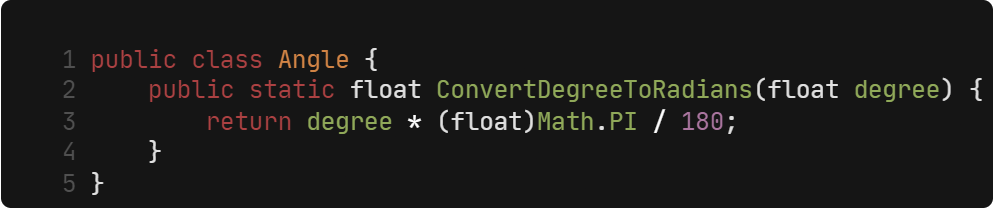
\includegraphics[width=\textwidth]{angle_class.png}
                \caption{Convertir grados a radianes.}
                \label{fig:angle_class}
            \end{figure}

        \subsection{Clase \textit{StraightLine}}

            \begin{figure}[H]
                \centering
                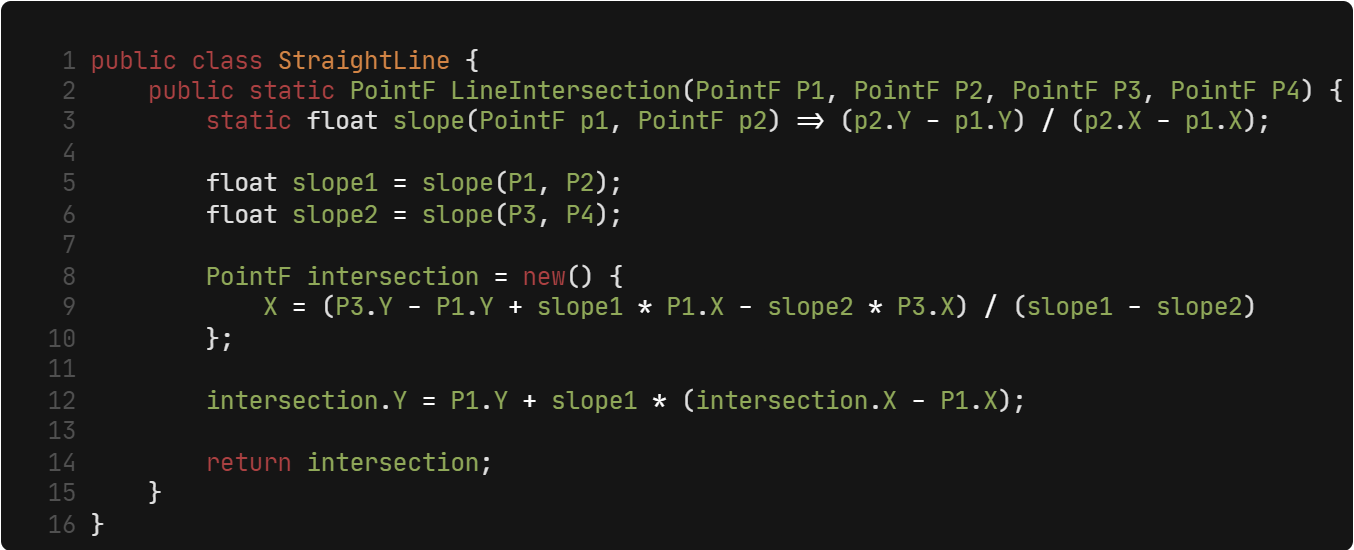
\includegraphics[width=\textwidth]{straight_line_class.png}
                \caption{Calcular punto medio entre dos rectas.}
                \label{fig:straight_line_class}
            \end{figure}

        \subsection{Clase \textit{Pentagon}}

            \begin{figure}[H]
                \centering
                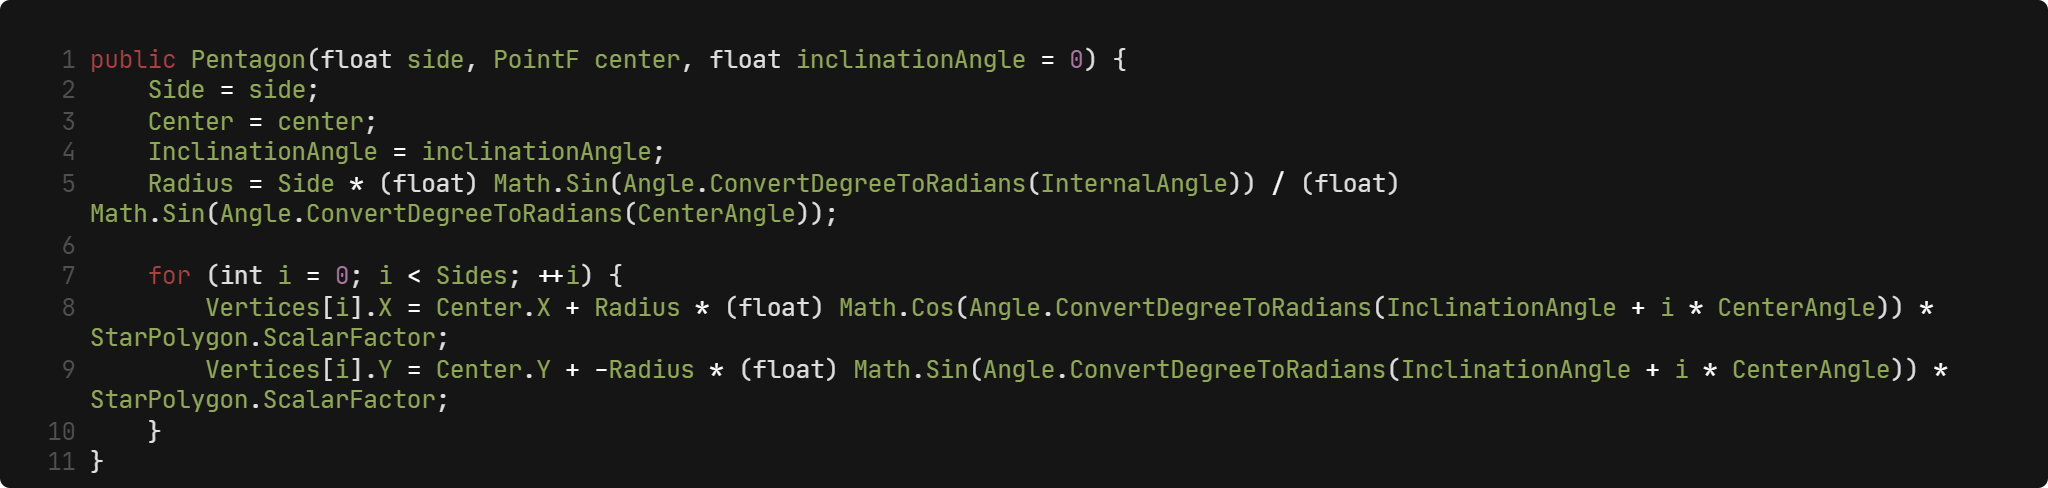
\includegraphics[width=\textwidth]{pentagon_constructor.png}
                \caption{Constructor de la clase \textit{Pentagon}.}
                \label{fig:pentagon_constructor}
            \end{figure}
            
            \begin{figure}[H]
                \centering
                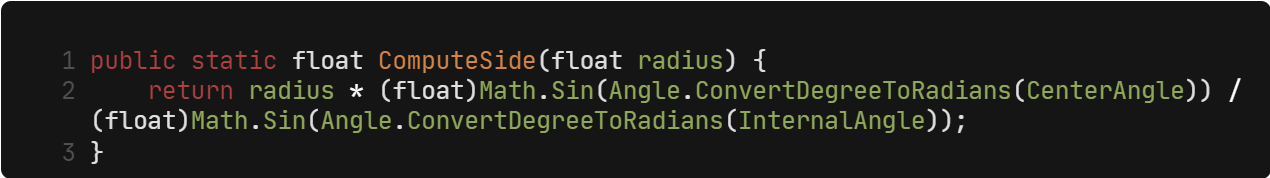
\includegraphics[width=\textwidth]{compute_side.png}
                \caption{Calcular lado del pentágono a partir del radio del círculo circunscrito.}
                \label{fig:compute_side}
            \end{figure}

            \begin{figure}[H]
                \centering
                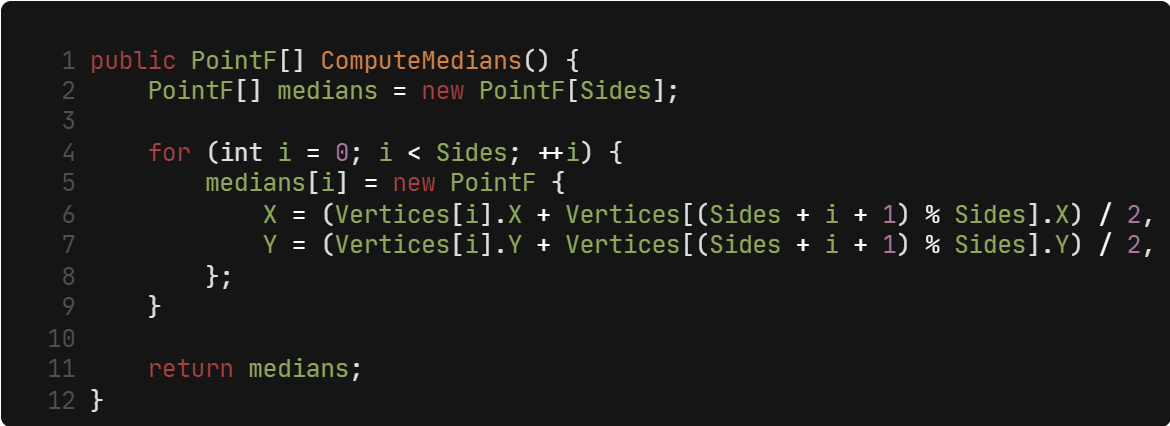
\includegraphics[width=\textwidth]{compute_medians.png}
                \caption{Calcular puntos medios de cada lado del pentágono.}
                \label{fig:compute_medians}
            \end{figure}

            \begin{figure}[H]
                \centering
                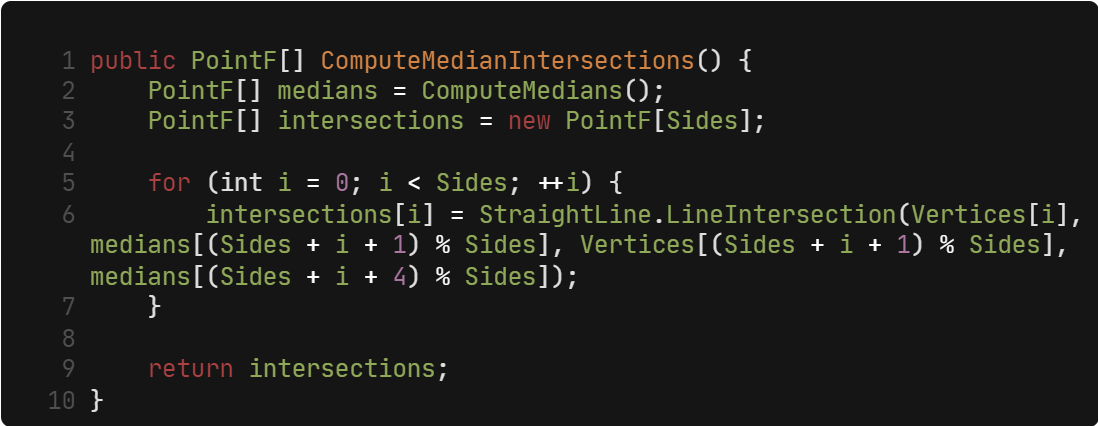
\includegraphics[width=\textwidth]{compute_median_intersections.png}
                \caption{Calcular puntos de intersección entre las medias del pentágono.}
                \label{fig:compute_median_intersections}
            \end{figure}

            \begin{figure}[H]
                \centering
                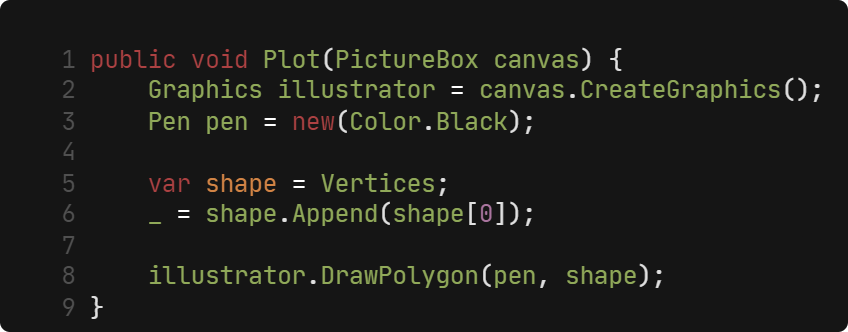
\includegraphics[width=\textwidth]{plot_pentagon.png}
                \caption{Graficar pentágono.}
                \label{fig:plot_pentagon}
            \end{figure}

            \begin{figure}[H]
                \centering
                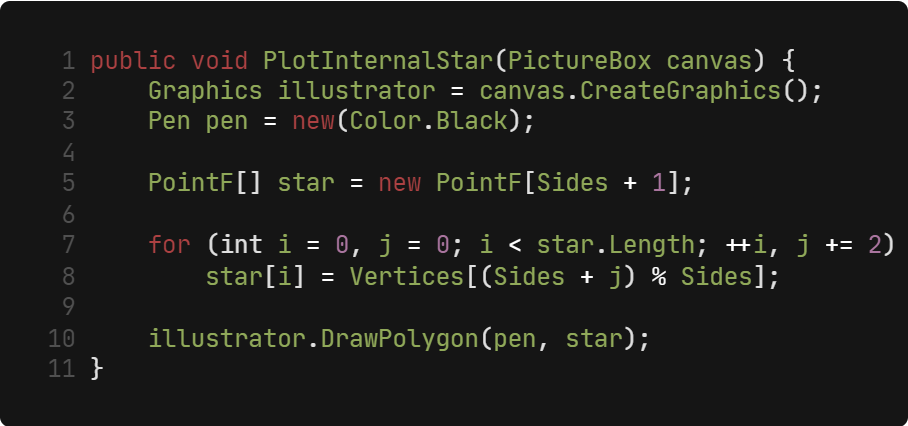
\includegraphics[width=\textwidth]{plot_internal_star.png}
                \caption{Graficar estrella interna de un pentágono.}
                \label{fig:plot_internal_star}
            \end{figure}

        \subsection{Clase \textit{StarPolygon}}

            \begin{figure}[H]
                \centering
                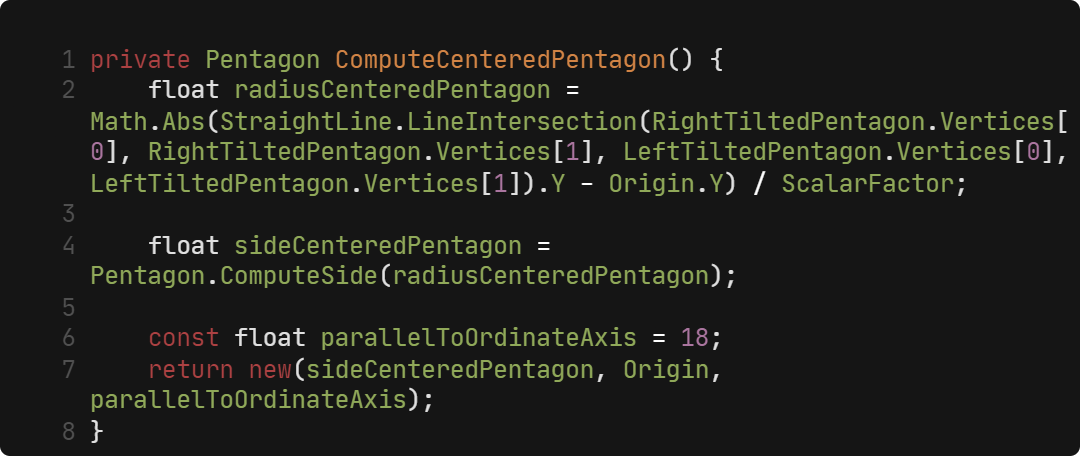
\includegraphics[width=\textwidth]{compute_centered_pentagon.png}
                \caption{Calcular medidas del pentágono central.}
                \label{fig:compute_centered_pentagon}
            \end{figure}

            \begin{figure}[H]
                \centering
                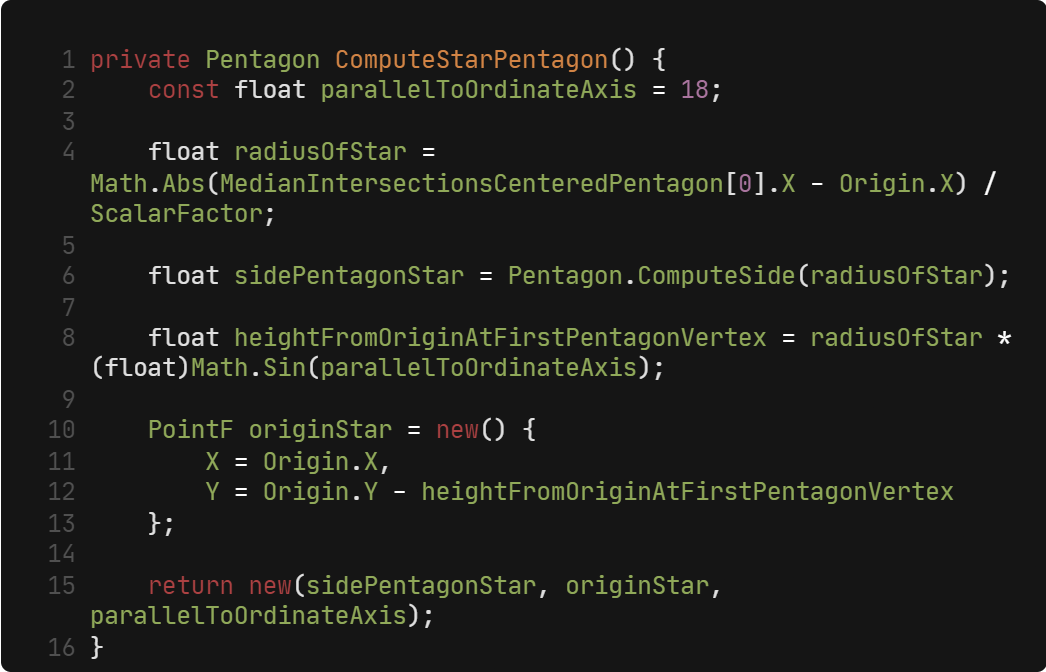
\includegraphics[width=\textwidth]{compute_star_pentagon.png}
                \caption{Calcular medidas de la estrella de 5 puntas central.}
                \label{fig:compute_star_pentagon}
            \end{figure}

            \begin{figure}[H]
                \centering
                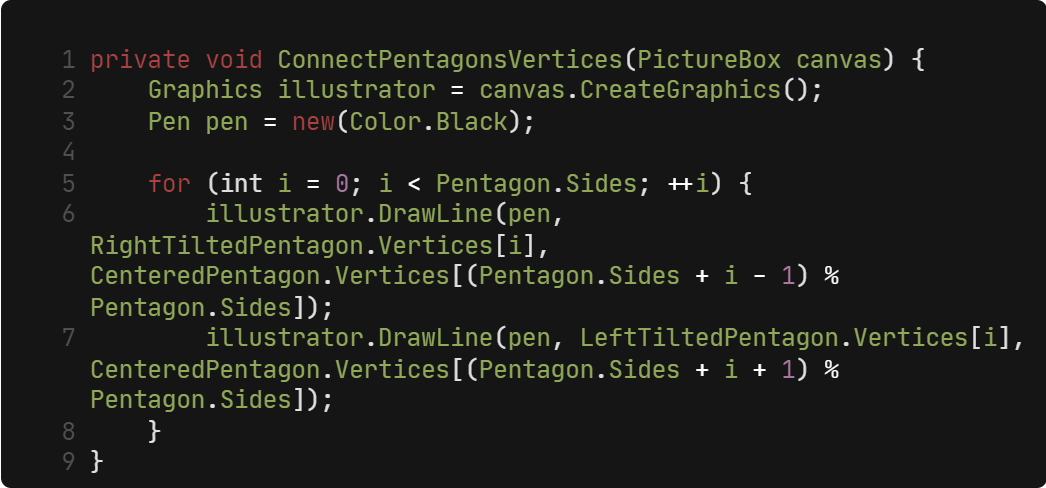
\includegraphics[width=\textwidth]{connect_pentagons_vertices.png}
                \caption{Unir los vértices de los pentágonos exteriores y el pentágono central.}
                \label{fig:connect_pentagons_vertices}
            \end{figure}

            \begin{figure}[H]
                \centering
                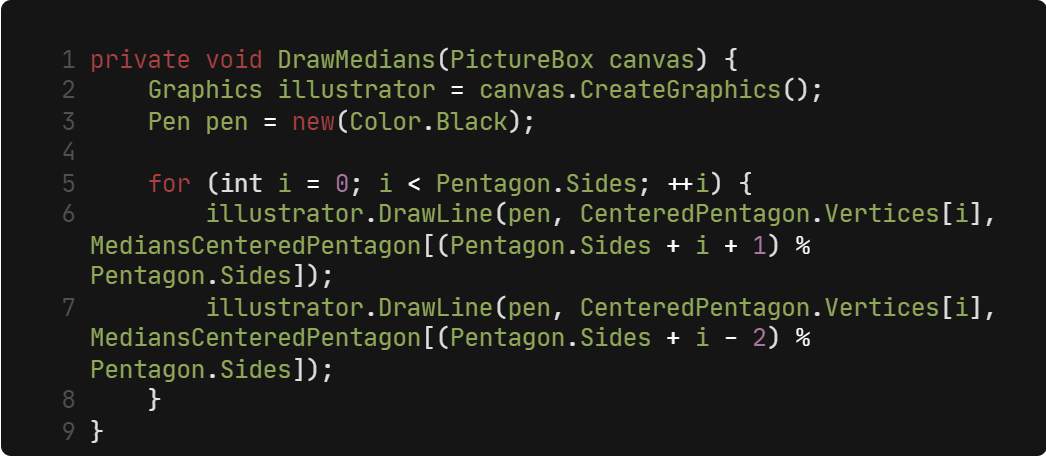
\includegraphics[width=\textwidth]{draw_medians.png}
                \caption{Dibujar medianas del pentágono central.}
                \label{fig:draw_medians}
            \end{figure}

            \begin{figure}[H]
                \centering
                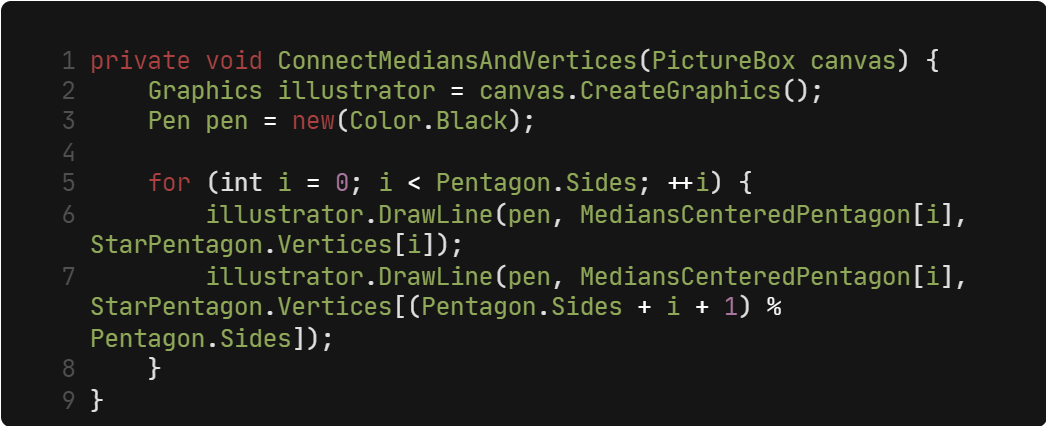
\includegraphics[width=\textwidth]{connect_medians_and_vertices.png}
                \caption{Unir medianas del pentágono central y vértices de la estrella de 5 puntas.}
                \label{fig:connect_medians_and_vertices}
            \end{figure}

            \begin{figure}[H]
                \centering
                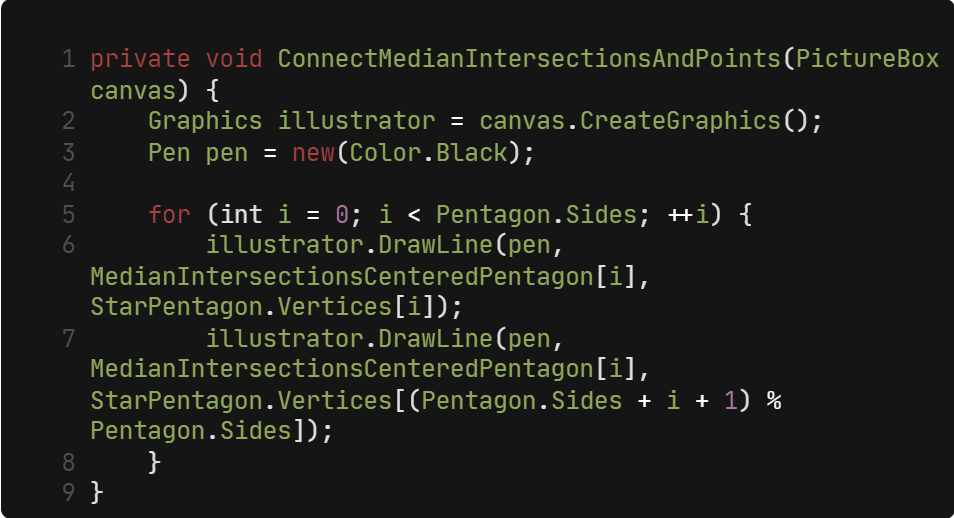
\includegraphics[width=\textwidth]{connect_median_intersections_and_points.png}
                \caption{Unir intersecciones de medianas del pentágono central y vértices de la estrella de 5 puntas.}
                \label{fig:connect_median_intersections_and_points}
            \end{figure}

            \begin{figure}[H]
                \centering
                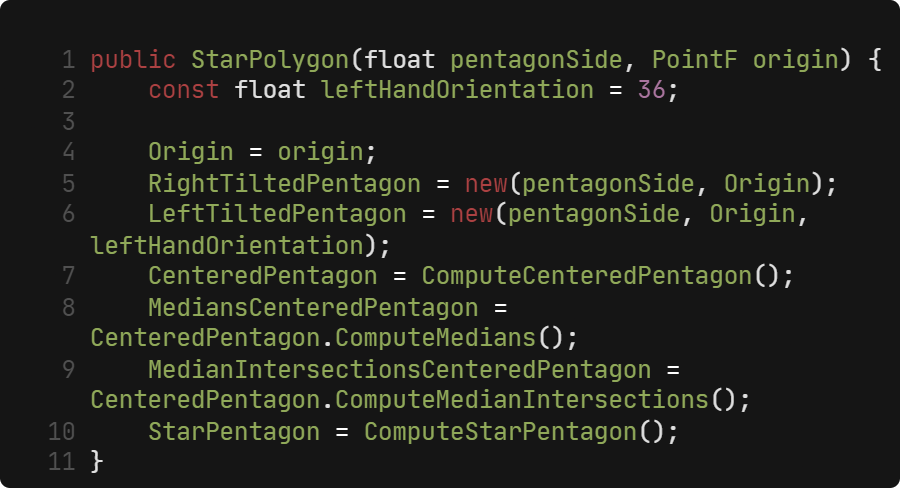
\includegraphics[width=\textwidth]{star_polygon_constructor.png}
                \caption{Constructor de la clase \textit{StarPolygon}.}
                \label{fig:star_polygon_constructor}
            \end{figure}

            \begin{figure}[H]
                \centering
                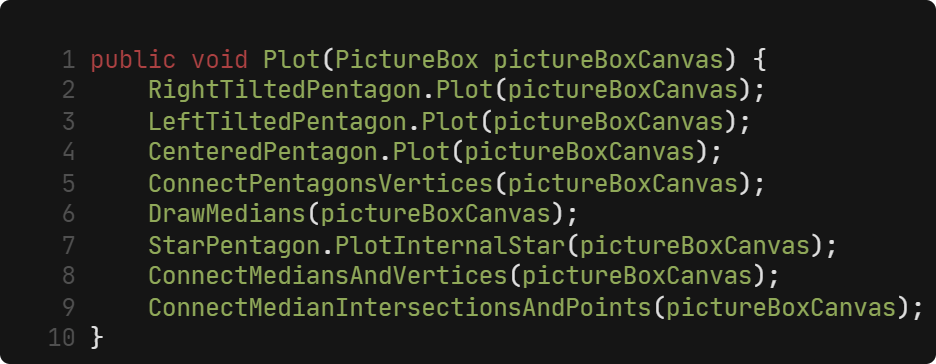
\includegraphics[width=\textwidth]{plot_star_polygon.png}
                \caption{Gráficar pentágonos y polígonos estrellados.}
                \label{fig:plot_star_polygon}
            \end{figure}

        \subsection{Clase \textit{Form1}}

            \begin{figure}[H]
                \centering
                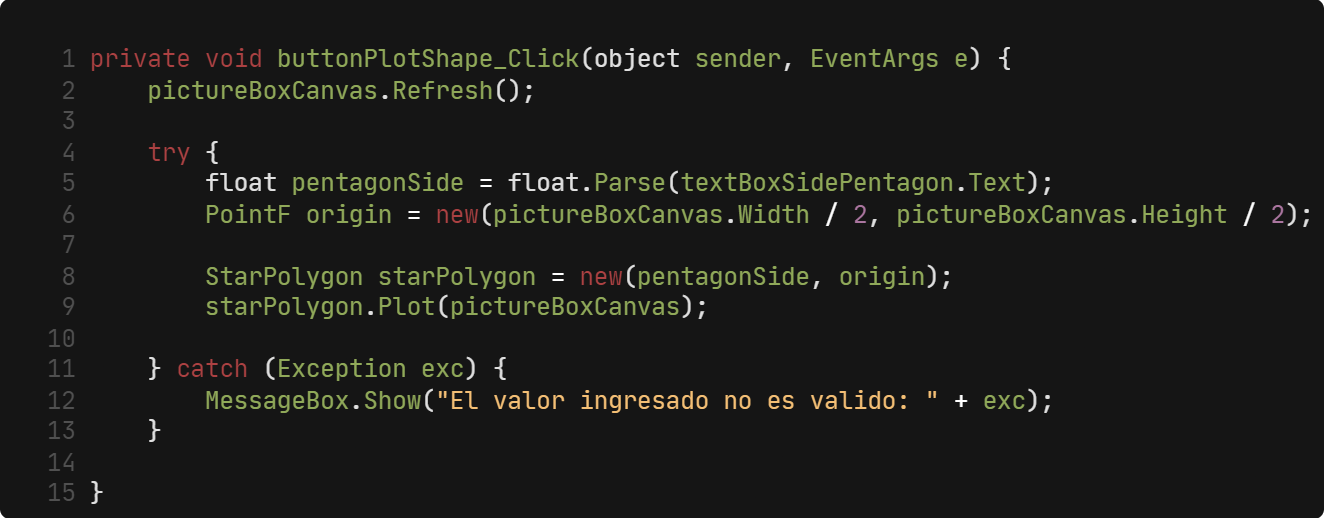
\includegraphics[width=\textwidth]{button_plot_shape.png}
                \caption{Función del botón ``Graficar''.}
                \label{fig:button_plot_shape}
            \end{figure}

    \section{Corrida del programa}

        \begin{figure}[H]
            \centering
            \includegraphics*[scale=0.5]{program_execution}
            \caption{Ejecución del programa.}
            \label{fig:program_execution}
        \end{figure}

\end{document}